\documentclass[technote]{IEEEtran}
%{{{ Packages
\usepackage[utf8]{inputenc}
\usepackage[T1]{fontenc}
\usepackage[scale=0.84]{geometry}
\usepackage[fleqn]{amsmath} 
\usepackage{amsthm,amssymb}
\usepackage{graphicx}
\usepackage{float}
\usepackage[caption=false,font=footnotesize]{subfig}
\usepackage{stfloats}
\usepackage{url}
\usepackage{caption}
\usepackage{lipsum}
\usepackage{multirow}
\usepackage{array}
\usepackage{listings}
\usepackage{color}
\usepackage{courier}
\renewcommand{\arraystretch}{1.5}
\def\thesectiondis{\thesection.} 
\def\thesubsectiondis{\Alph{subsection}.} 
\lstset{language=C++,
    keywordstyle=\color{blue},
    stringstyle=\color{red},
    commentstyle=\color{green},
    morecomment=[l][\color{magenta}]{\#}
}
%}}}
%{{{ Title
\begin{document}
\begin{titlepage}
    \vspace*{\fill}
    \begin{center}
        \usefont{T1}{cmr}{m}{n}
        {\Huge CSCI-2100 Data Structures Lab}\\[0.3cm]
        {\huge Profiling Dijkstra's Algorithm}\\[0.6cm]
        {\Large Chad Chapnick}\\[0.4cm]
        {\small\today}
    \end{center}
    \vspace*{\fill}
\end{titlepage}
%}}}
\section{Introduction}

Dijkstra's algorithm addresses the problem of 
the minimum distance from a source vertex, $v$, to every 
other vertex in the graph. 

%This is a question about the global 
%structure of the graph.

Dijkstra's algorithm requires a subroutine which returns 
the index of the univisted vertex which is closest to the source vertex.
For this analysis, we will refer to this subroutine as \texttt{minVertex}.

The pseudocode is outlined as follows:
\begin{lstlisting}
D := array of best known distances from v
     to every other vertex
while (there exist unvisited verticies):
    call minVertex, returns a vertex v.
    mark v as visited.
    for each neighbor, w, of v:
        if D[w] > D[v] + weight(v, w):
            D[w] = D[v] + weight(v, w)
\end{lstlisting}





A trivial implementation of \texttt{minVertex} can be achieved by linearly 
searching through the array of best known distances, and returning the 
index of the unvisited vertex with the smallest value. 
The time complexity of this implementation is described by:

$$\Theta(|V|^2 + |E|)$$

where the $|E|$ term arises from the fact that we visit each edge once.

\subsection{Comparison}
%In this context, the density graph is defined as \_\_\_. 

From this we can see that if $|E| \in |V|$, 
then the upper bound for the run time is $O(|V|^2)$.


The use of a binary-heap in \texttt{minVertex} yields a 
lower time complexity on average relative to the linear implementation


%For intuition, this can be which can be though of 
%as $\Theta(|V|)$ for |V| vertices.

%the distances are stored in a -heap.

This can be broken down into two components. 
The $|V|\log|E|$ term comes from the fact that for every vertex, 
we must call the \texttt{minVertex} function.
The $|E|\log|E|$ term is the cost of adding an element to the 
heap for every edge (worst case).

The total runtime is 
$$\Theta ( (|V| + |E|) \cdot \log|E| )$$


To understand the asymptotic performance of this algorithm, 
we need to consider a few cases.
If $|E|$ is bounded above by $|V|$, (ie. $|E| \in O(|V|)$), 
then the linear implementation is $\Theta(|V|^2)$, 
and the heap implementation is $O(|V| \log |V|)$.



\section{Results}

An analysis of each implmentation was tested for 
three cases, namely: 

%$$
%\begin{cases}
    %|E| = |V| - 1\\
    %|E| = |V|  \\
    %|E| = |V|(|V| - 1)/2
%\end{cases}
%$$




\begin{figure}[ht!]
    \centering
    \caption{\label{fig:runtimePlots} Runtime for Dijkstra's Algorithm}
    \subfloat[]{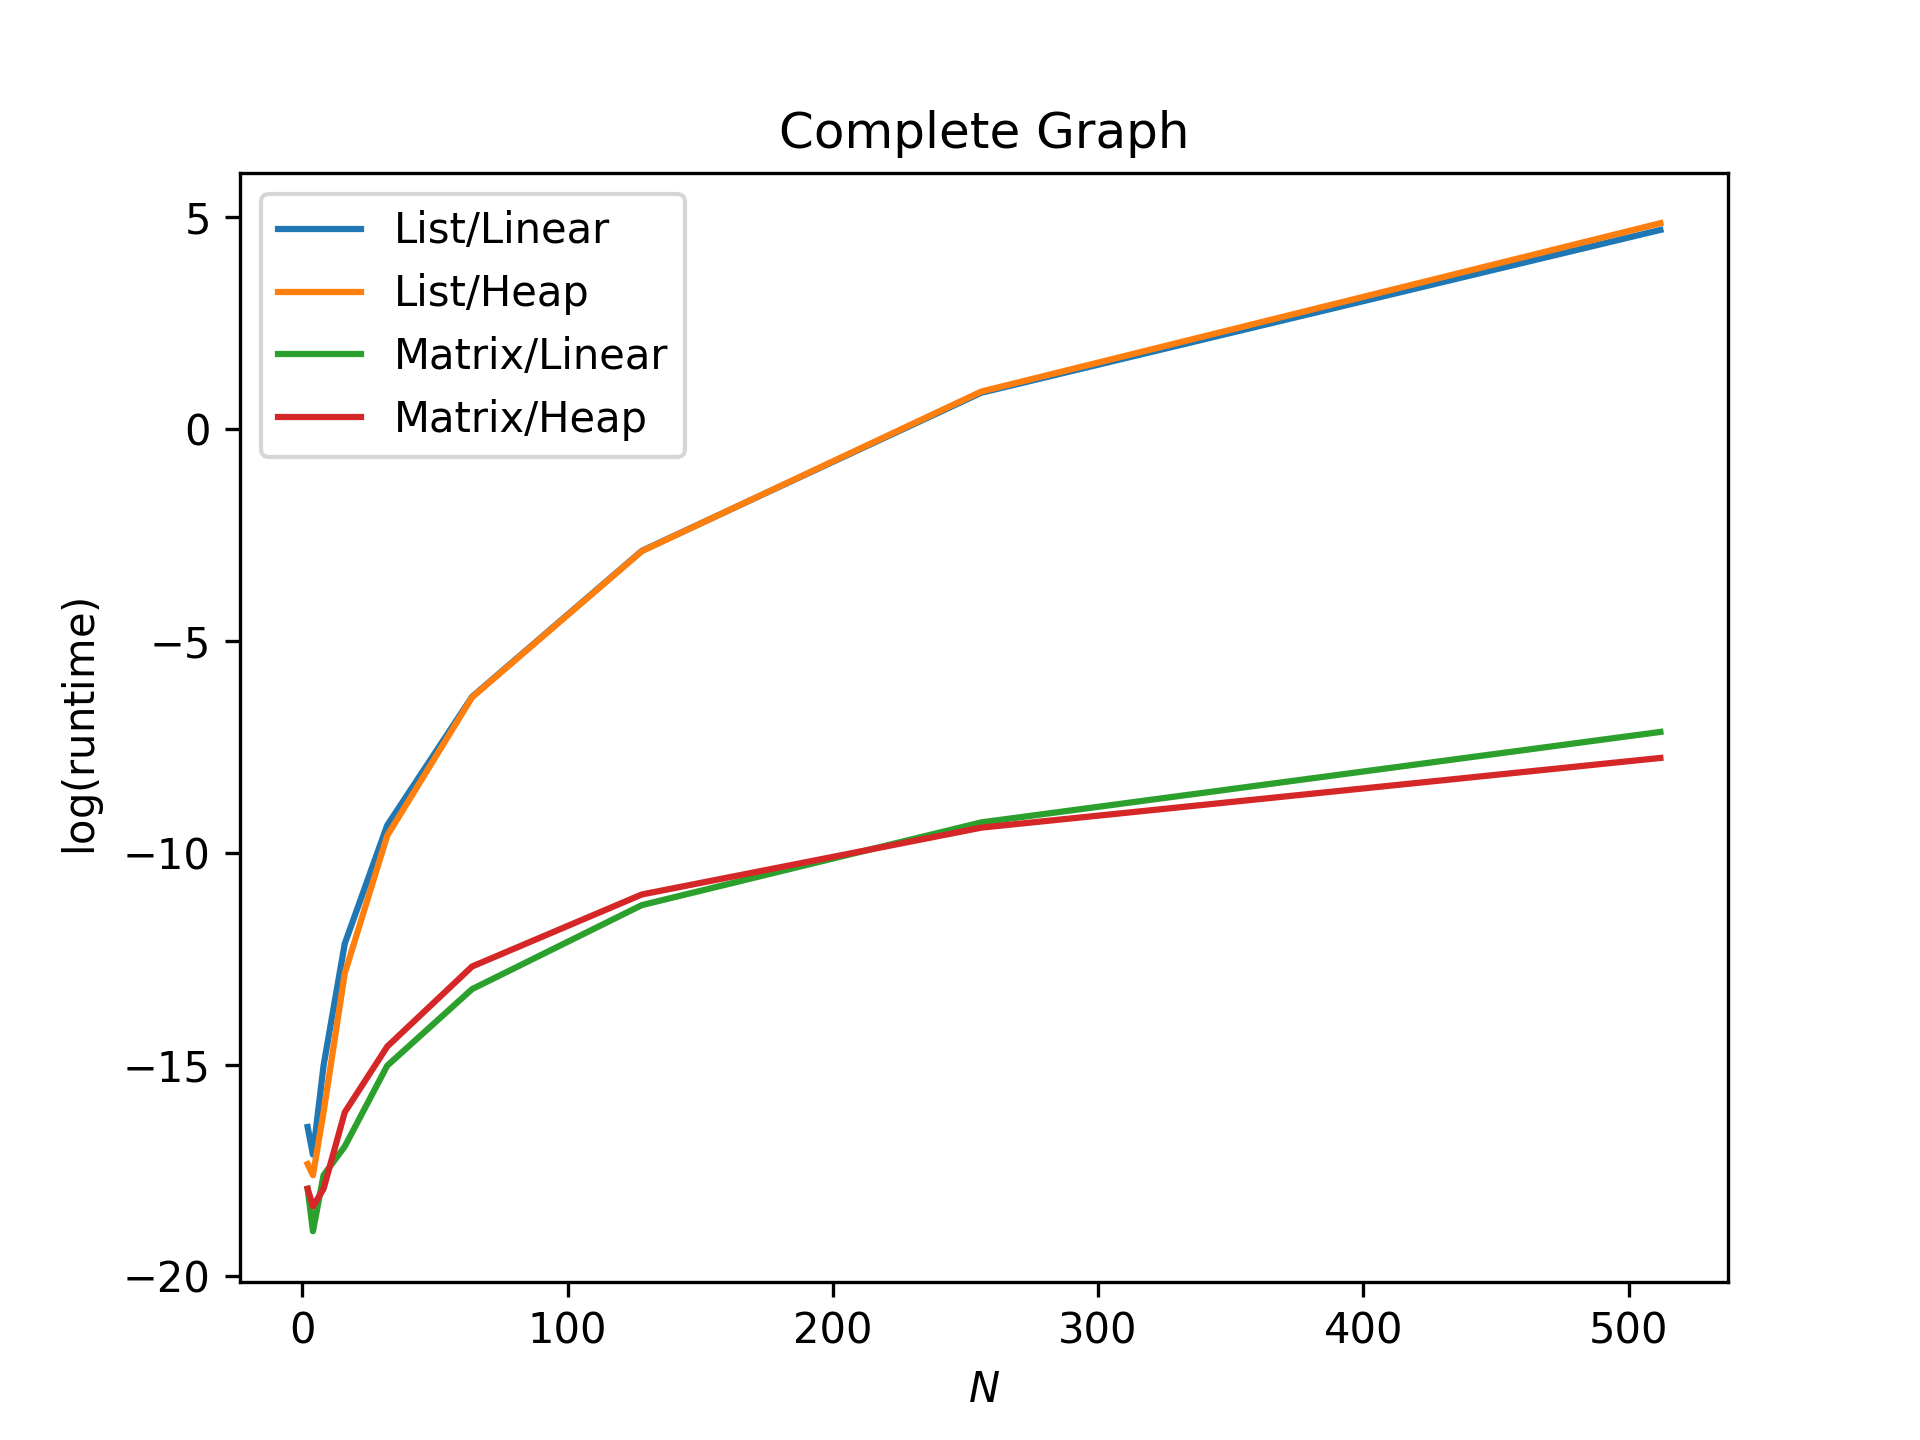
\includegraphics[width=\columnwidth]{./figure0.png}}

    \subfloat[]{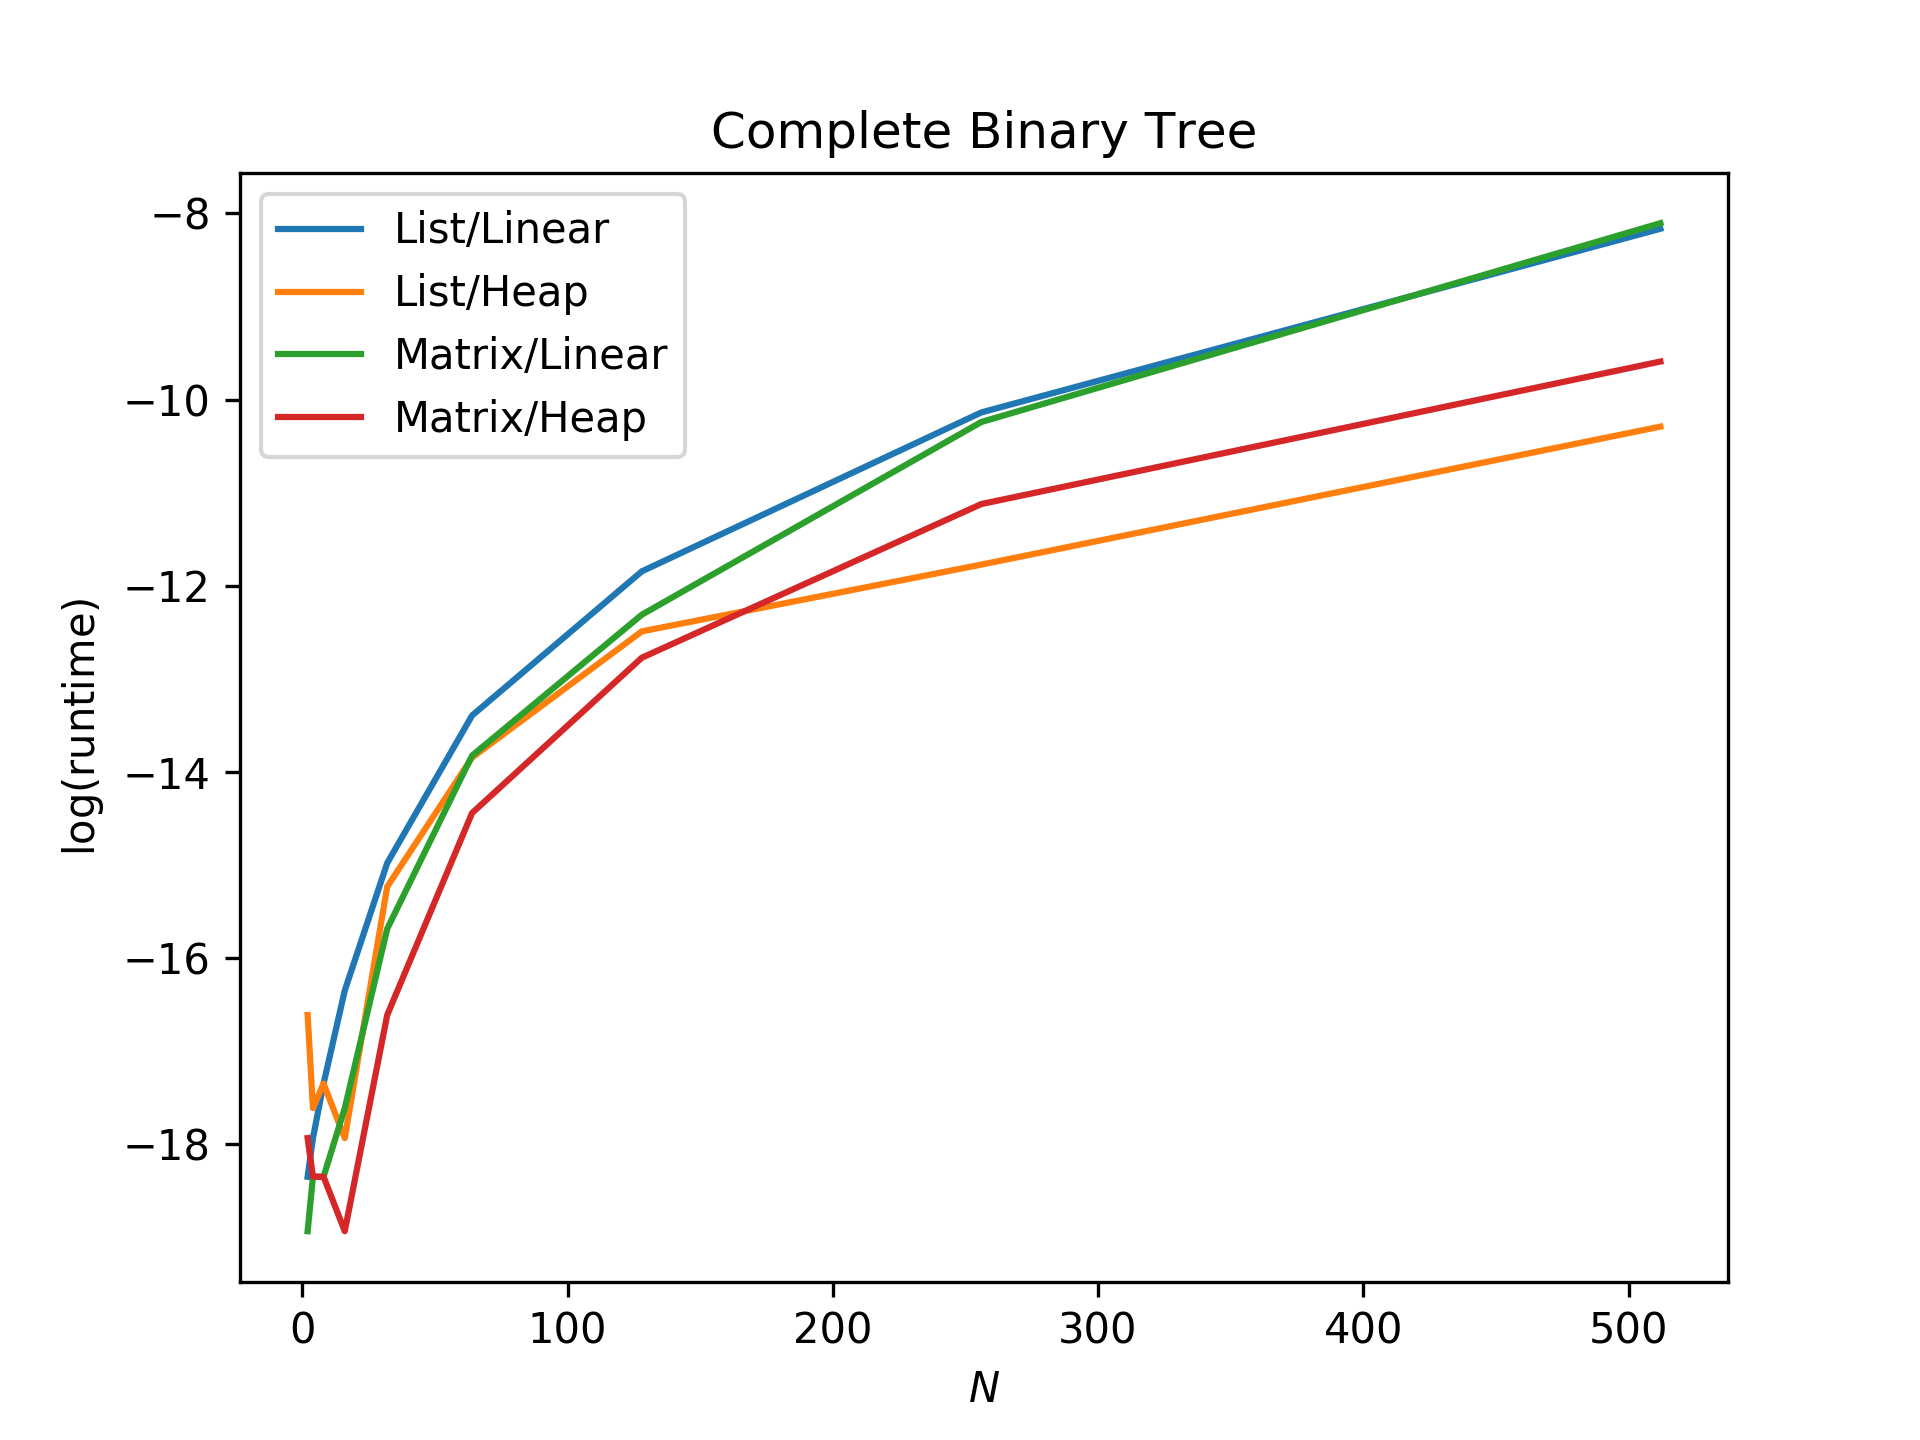
\includegraphics[width=\columnwidth]{./figure1.png}}

    \subfloat[]{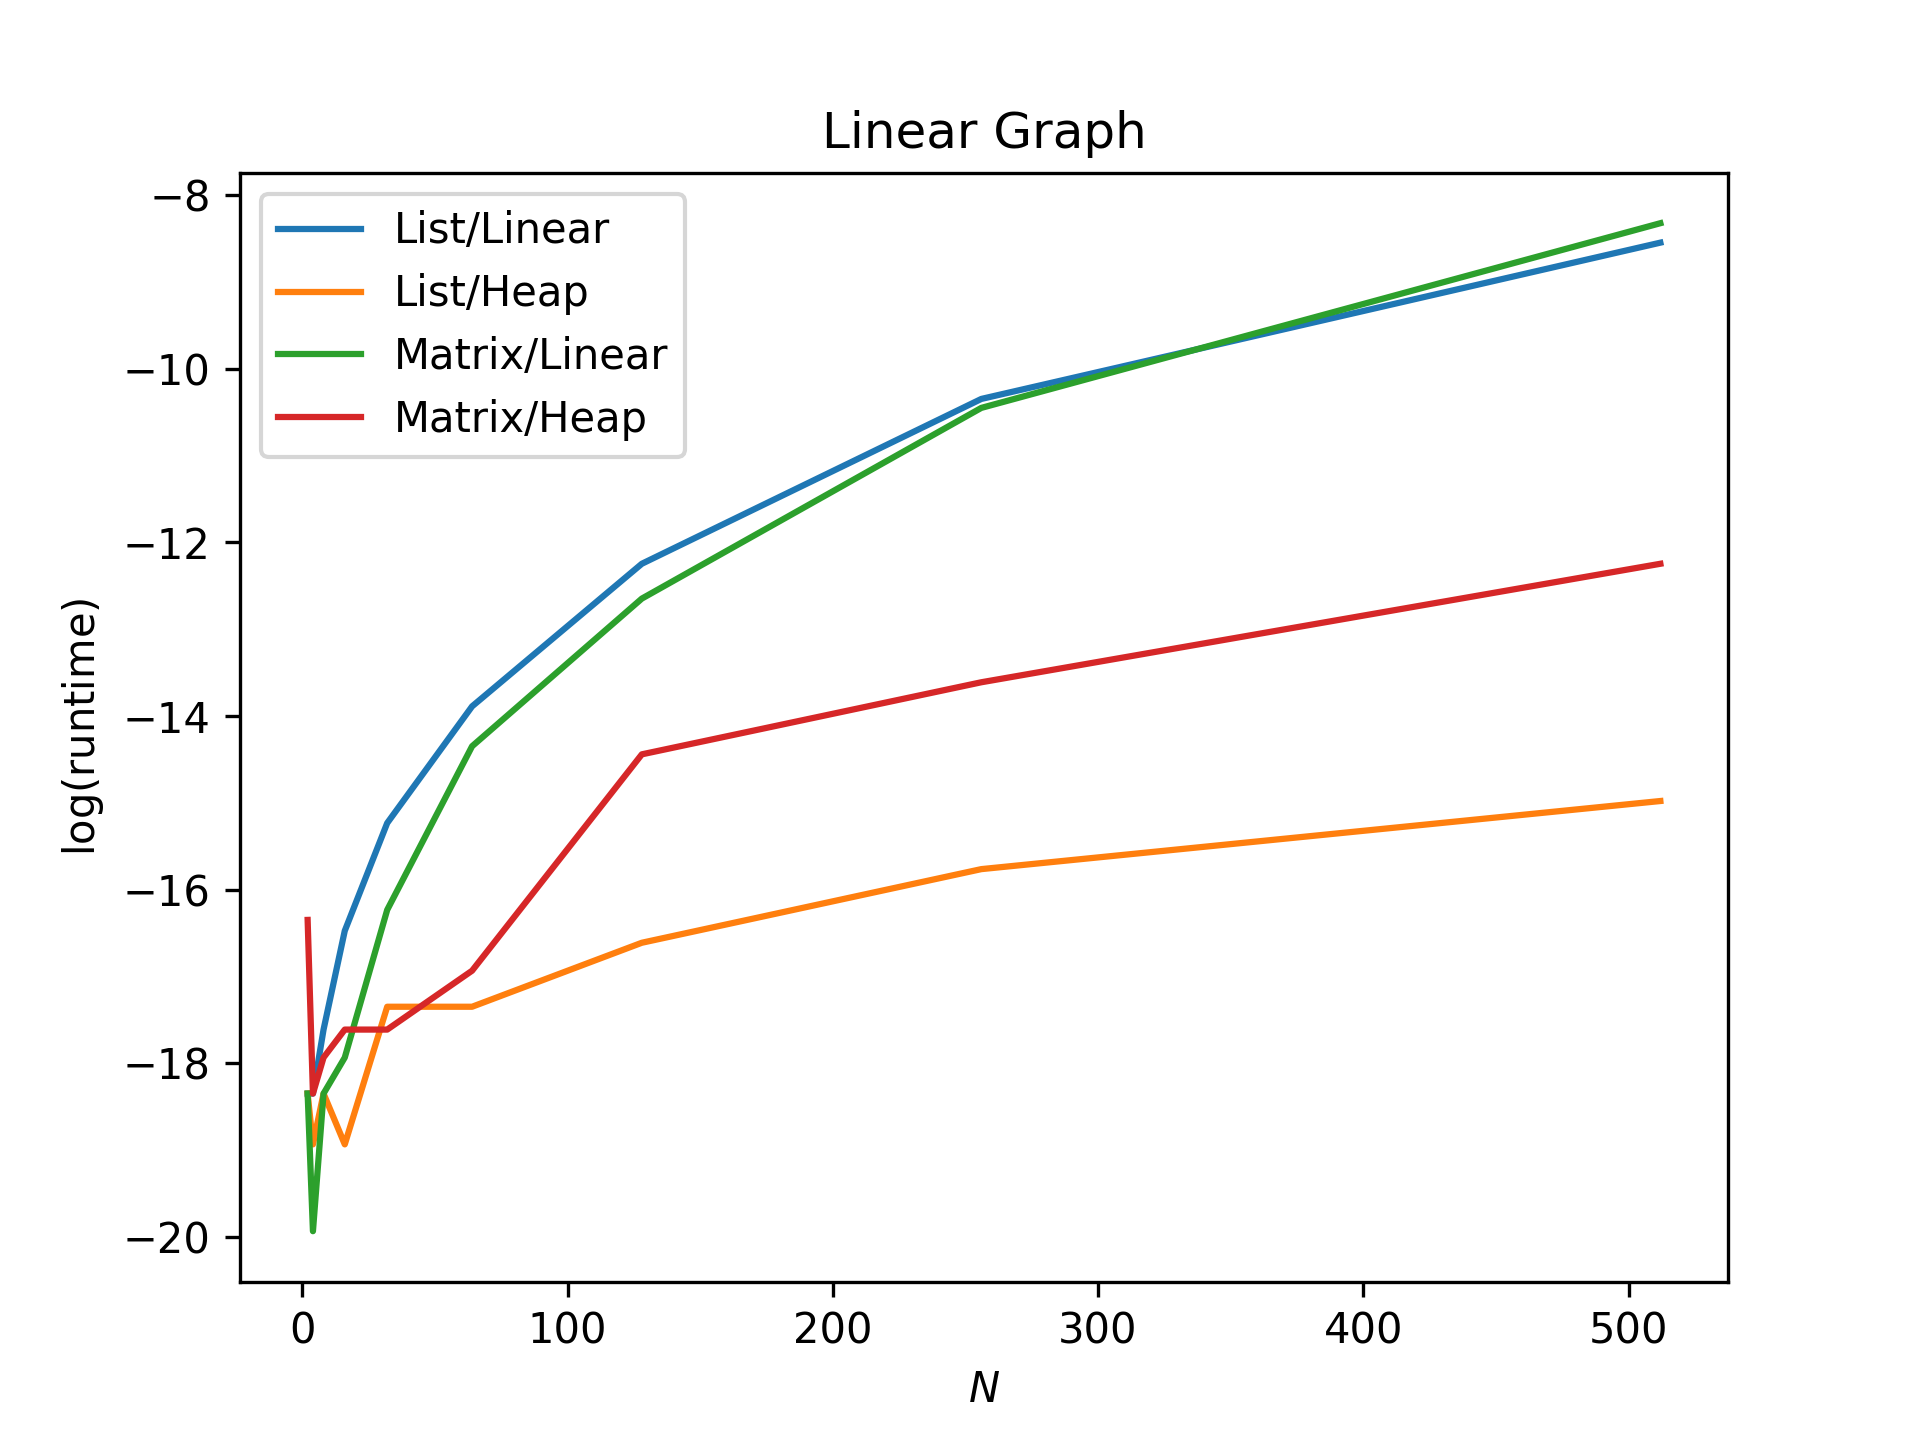
\includegraphics[width=\columnwidth]{./figure2.png}}
\end{figure}


\begin{table}[!ht]
    \caption{Runtimes}
    \centering
    \begin{tabular}{|c|c|c|c|}
        \hline
        & DENSITY & LINEAR & HEAP \\ \hline
        \multirow{3}{*}{Adjacency List} 
        & Linear Graph & 0.0 & 0.0 \\ [0.5ex]\cline{2-4}
        & Complete Binary Tree & 0.0 & 0.0 \\ \cline{2-4}
        & Complete Graph & 0.0 & 0.0 \\ \hline
        \multirow{3}{*}{Adjacency Matrix}
        & & 0.0 & 0.0 \\ \cline{2-4}
        & & 0.0 & 0.0 \\ \cline{2-4}
        & & 0.0 & 0.0 \\ \hline
    \end{tabular}
\end{table}


%\begin{figure*}[hb!]
    %\caption{Nodes of Dublin}
    %\centering
    %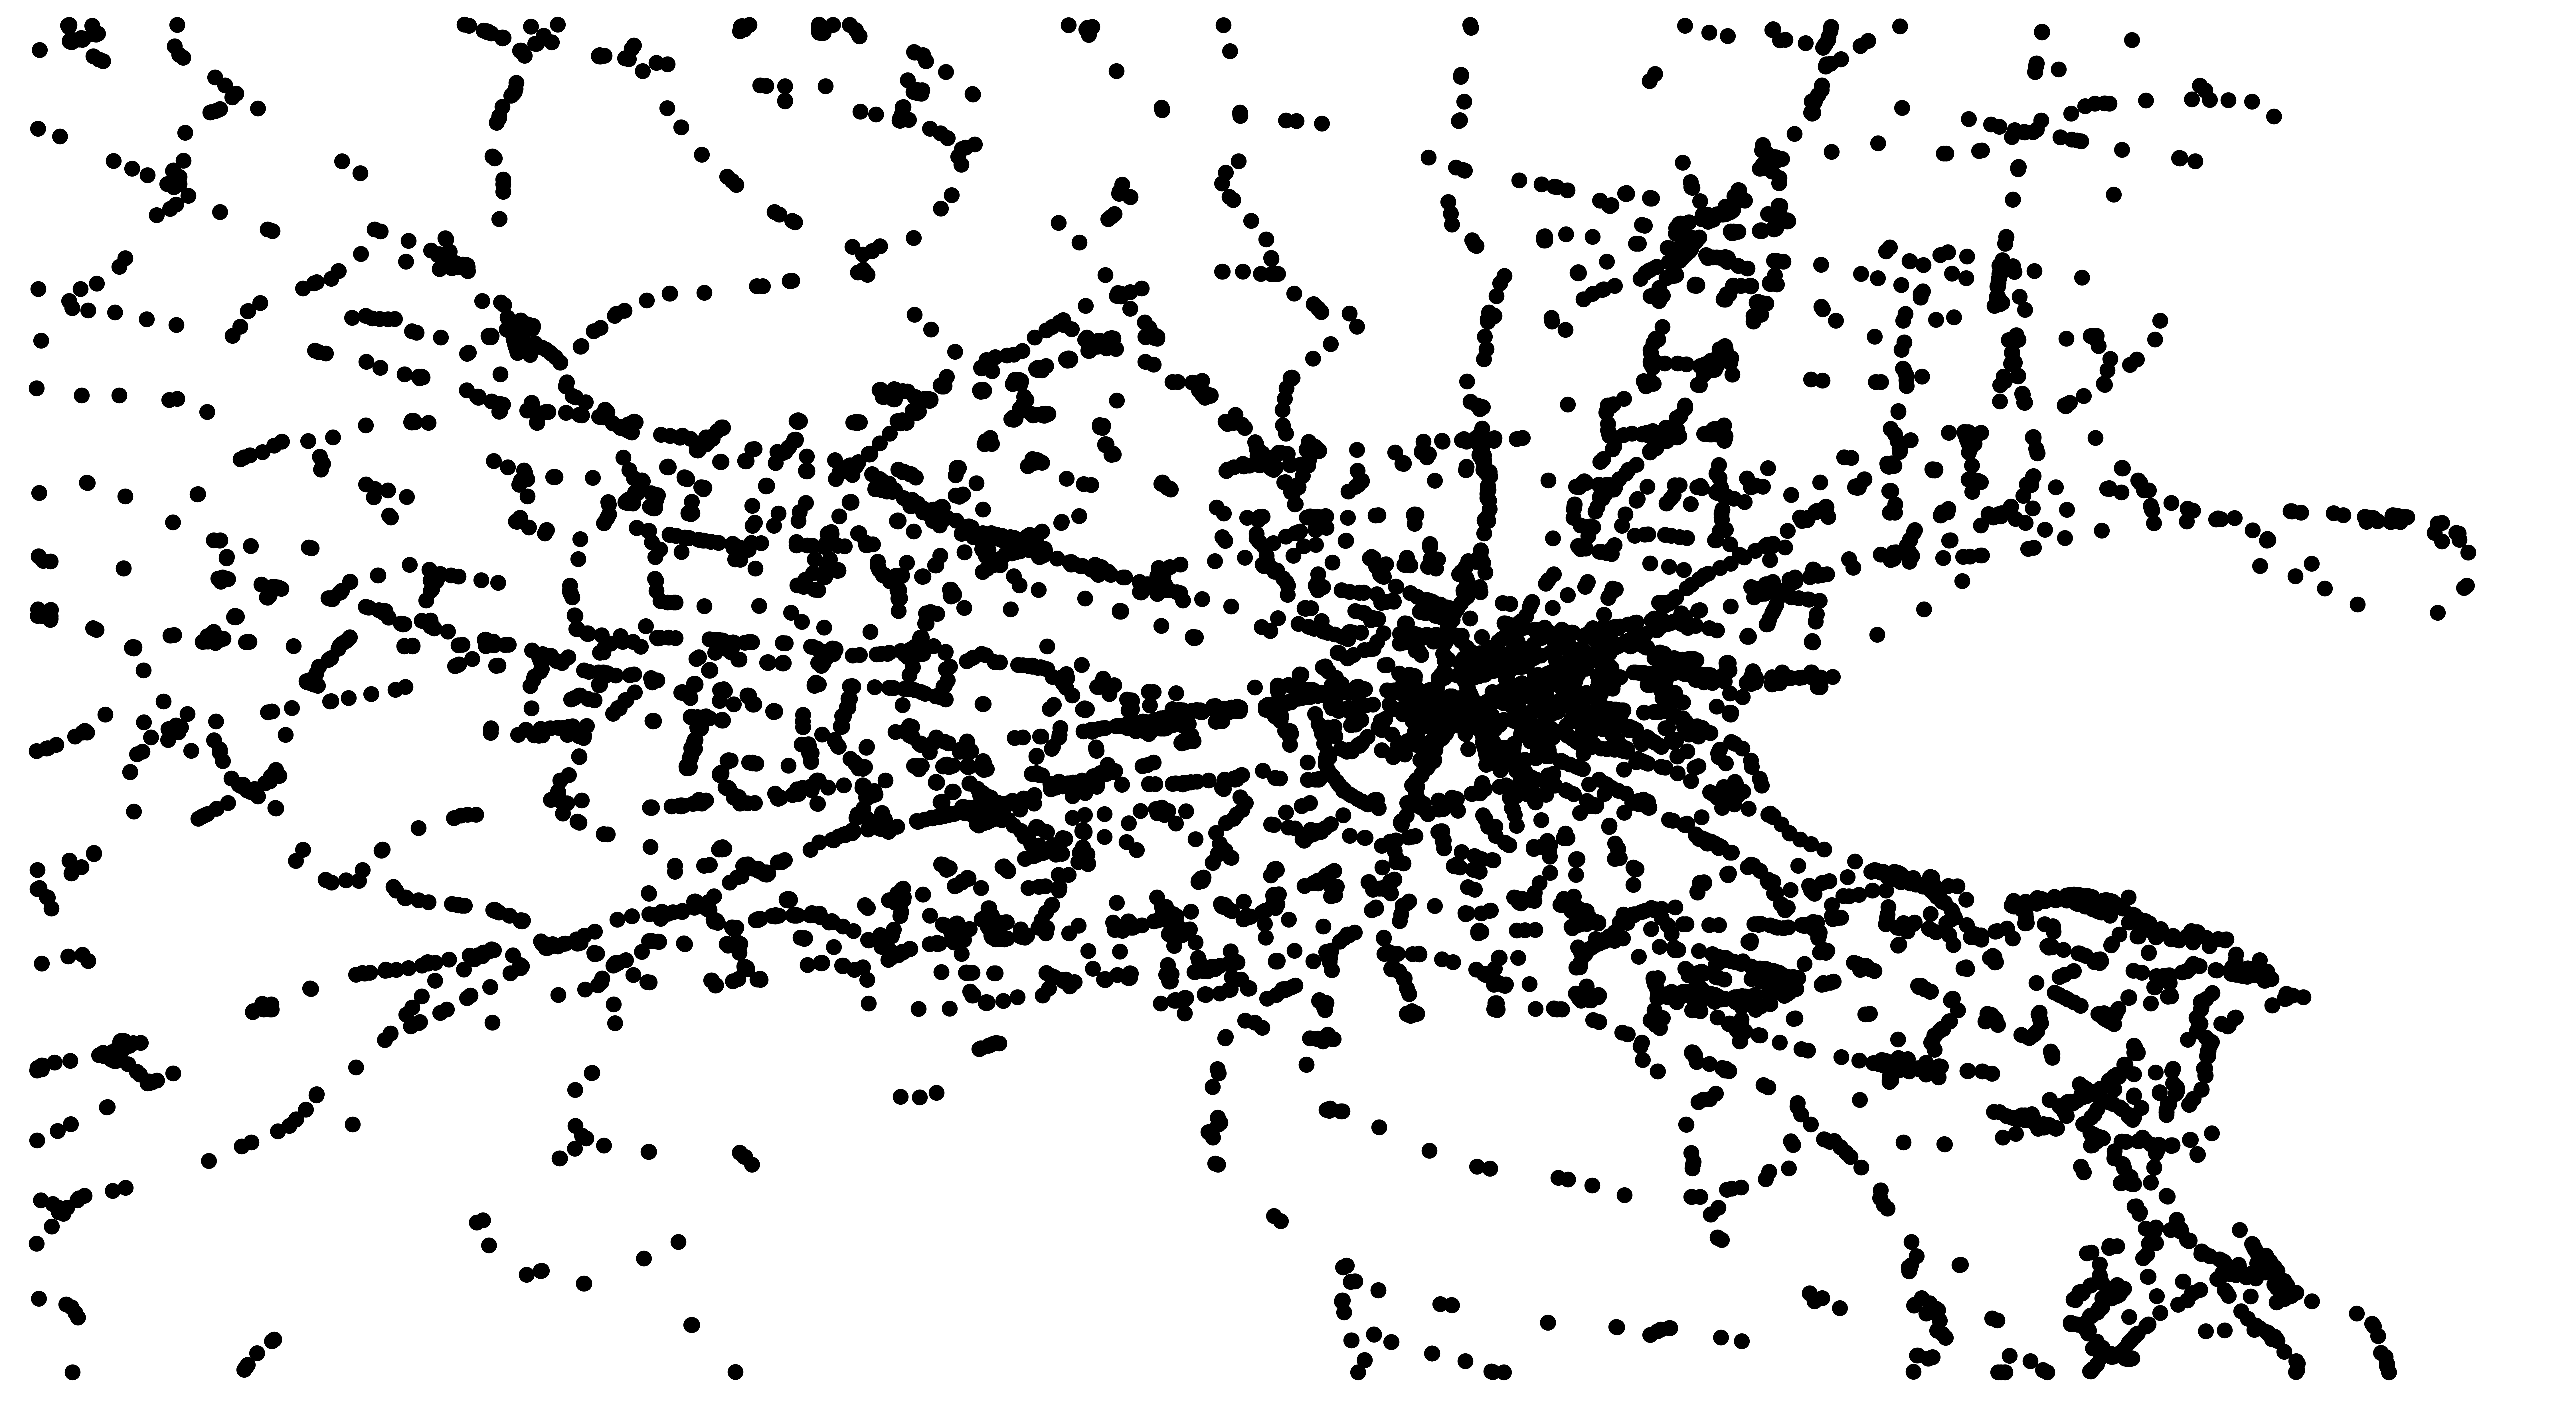
\includegraphics[width=0.75\textwidth]{scatter.png}
%\end{figure*}





\section{Conclusion}
If  E is sufficiently smaller compared to V (as in E << V² / logV), then using heap becomes more efficient.

\lipsum[1-2]

%{{{    Bibliography
\nocite{*}
\bibliographystyle{IEEEtran}
\bibliography{references.bib}
%}}}
\end{document}
